\chapter{Theory}

\section{Helical resonator models}
In order to create a helical resonator satisfying our experimental conditions and limitations we inevitably come to a need for a theoretical model that would be able to predict the essential characteristics of the resulting unit. The following sections aim to provide an overview and comparison between the models.

\subsection{Macalpine \& Schildknecht}
\begin{figure}[h]
	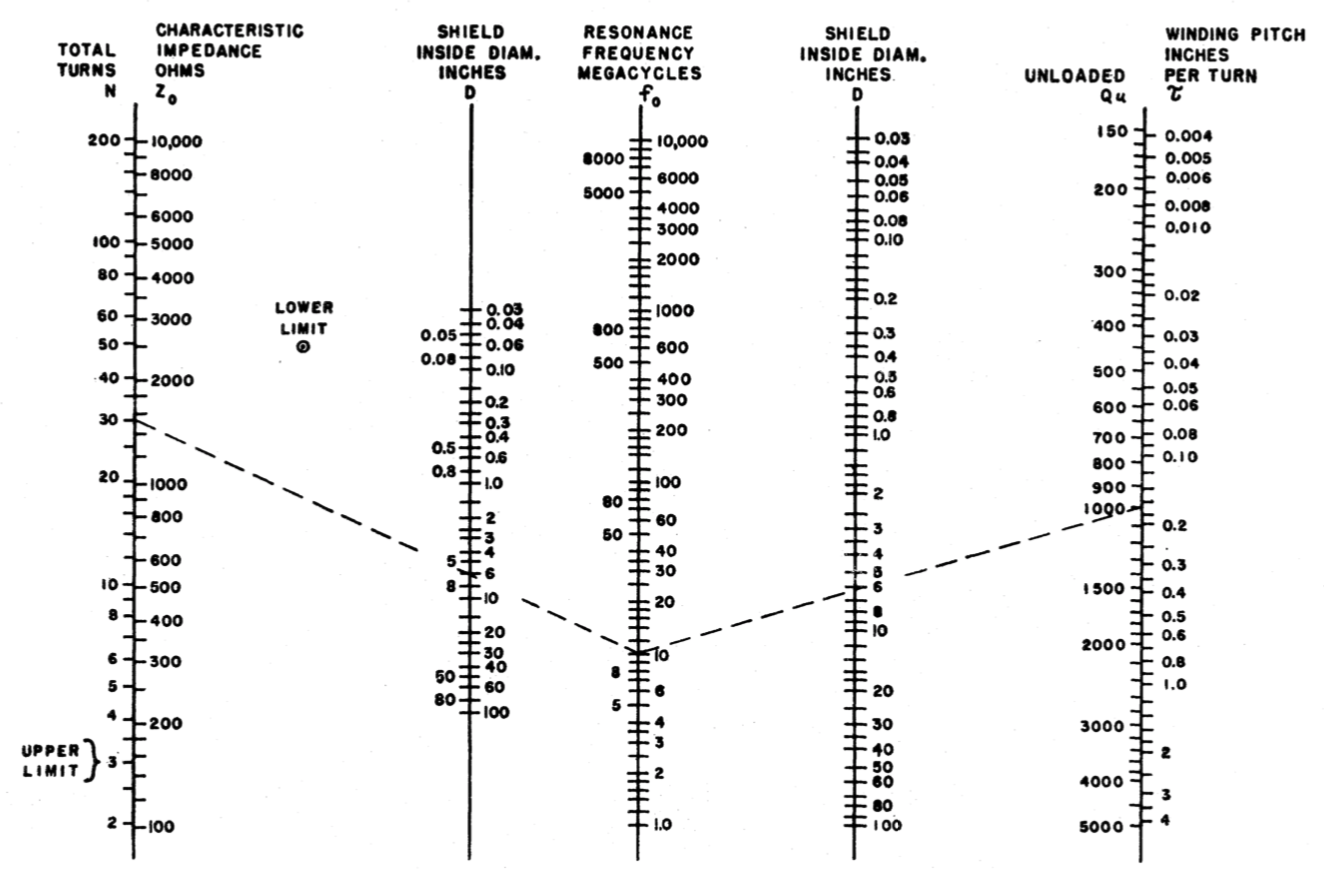
\includegraphics[width=\textwidth]{images/macalpine_chart}
	\caption{Design chart for quarter-wave helical resonators.}
	\label{fig:macalpine_chart}
\end{figure}

A well-known approach \cite{Macalpine2000} for describing helical resonators was introduced in the same year as Richard Feynman's idea \cite{Feynman1960} to use quantum systems for computations. It was motivated by the possibility to reduce volume compared to TEM-mode coaxial-line resonators. While skipping a detailed theoretical analysis it nevertheless provides a basis for constructing a resonator: such as regions of usefulness, design considerations and a set of parameters' dependencies maximizing $Q$.

While describing essential properties of an unloaded helical quarter-wave resonator this paper \cite{Macalpine2000} also predicts the shift of resonant frequency if an external load is connected. In order to define a new frequency one can make use of telegraph equations \cite{Rohde2009} by effectively treating the ion trap as a capacitor.

\subsection{Siverns et al.}
Unfortunately modeling an ion trap as a pure capacitive load is not always accurate. Introducing resistive losses imposes an additional shift of resonant frequency which pushes the deviation from self-resonant frequency even further. It is possible to tune the strength of the inductive coupling between the antenna and the main coil to compensate this shift while losing in efficiency.

These limitations of Macalpine's \& Schildknecht's \cite{Macalpine2000} model have been overcome in a newer paper \cite{Siverns2012} which takes the development of an amplifier, specifically for the needs of quantum computing, one step further. By taking a look at the joint resonator + ion trap system as a whole it aims to predict the effective $Q$ and frequency. This model ensures that it's possible to find optimal parameters for given experimental constraints.

\section{Comparison}
Macalpine's and Schildknecht's \cite{Macalpine2000} model gives insides for designing a helical quarter-wave resonator with a given self-resonant frequency. However major shifts from it can be expected when connecting the ion trap. Siverns' et al. approach \cite{Siverns2012} investigates connections between various parameters in the total circuit. As a result one could create a resonator which implements a transfer function closer to a desired one. Considering these benefits the Siverns model \cite{Siverns2012} was selected.